% Generated from the canonical English manuscript; compile with pdfLaTeX twice.
\documentclass[11pt,a4paper]{article}
\usepackage[T1]{fontenc}
\usepackage[utf8]{inputenc}
\usepackage{lmodern}
\usepackage[margin=25mm]{geometry}
\usepackage{amsmath,amssymb}
\usepackage{graphicx}
\usepackage{booktabs,array,tabularx}
\usepackage[font=small,labelfont=bf,labelsep=period]{caption}
\usepackage[unicode,hidelinks]{hyperref}
\urlstyle{same}
\setlength{\emergencystretch}{2em}
\setlength{\parskip}{3pt}
\setlength{\textfloatsep}{16pt plus 3pt minus 3pt}
\setlength{\intextsep}{14pt plus 3pt minus 3pt}
\renewcommand{\topfraction}{0.90}
\renewcommand{\bottomfraction}{0.85}
\renewcommand{\textfraction}{0.08}
\renewcommand{\floatpagefraction}{0.65}
\providecommand{\tightlist}{\setlength{\itemsep}{0pt}\setlength{\parskip}{0pt}}
\raggedbottom
\hypersetup{pdftitle={QwenQPU A Language Model with an Internal Quantum Circuit Simulator},pdfauthor={OpenQuantum}}
\begin{document}
\begin{center}
{\LARGE\bfseries QwenQPU A Language Model with an Internal Quantum Circuit Simulator\par}
\vspace{12pt}
{\large OpenQuantum\par}
\vspace{8pt}
\end{center}
\begin{abstract}
We present QwenQPU, a language model with a quantum-circuit simulator implemented within its standard layers. The model combines 32 language layers inherited from Qwen3.5-4B with four analytically constructed, fixed-weight layers. The language layers produce structured requests; the execution layers maintain addressable complex amplitudes in recurrent state, compose quantum gates through shared SwiGLU arithmetic, and correct probability readout under a specified norm condition. The added operators require no further training and run through the standard Transformers forward pass. We evaluate 48 frozen, paired tasks spanning 3, 4, and 6 logical qubits and 12, 18, and 24 sequential gates. Both conditions share language weights and a budget ceiling of 16,384 generated predictions, including every QPU forward prediction. Enabling execution increases the number of tasks satisfying an absolute error threshold of 5\ensuremath{\times}10\textsuperscript{-5} for both requested event probabilities from 4/48 to 48/48. The maximum probability error is 1.42\ensuremath{\times}10\textsuperscript{-5}, with a two-sided exact McNemar p-value of 1.14\ensuremath{\times}10\textsuperscript{-13}. Under the fixed six-qubit, two-event protocol, QPU predictions follow \(N_{\mathrm{QPU}}=2{,}063+514G\), where G is the gate count; improved task success comes with more total predictions and longer runtime. These results demonstrate an executable and verifiable integration of explicit numerical rules with pretrained language capabilities, with accuracy and cost characterized within a finite-capacity, finite-precision setting.
\end{abstract}
\textbf{Keywords:} large language models; quantum circuit simulation; compiled weights; Gated DeltaNet; numerical execution; reproducible evaluation

\section{Introduction}

Language models used for scientific computation must translate natural-language requirements into verifiable numerical results. Toolformer learns to invoke external APIs \cite{ref1}, PAL and Program of Thoughts delegate computation to program interpreters \cite{ref2}, \cite{ref3}, and ReAct organizes sequences of reasoning and interaction with an environment \cite{ref4}. These approaches highlight the importance of reliable execution. Here we ask whether explicit state-transition rules can be incorporated into a language model's standard forward computation to complete tasks that require continuously updated numerical state, subject to a specified error tolerance.

We introduce QwenQPU, which implements a state-vector simulator with a capacity of six qubits in four fixed-weight QPU layers and combines them with 32 inherited language layers in a single model. The language layers formulate circuit-execution requests; the QPU layers update complex amplitudes according to the gate sequence and return the probabilities of specified events. The design connects addressable state, gate arithmetic shared across addresses, and finite-precision readout into one execution path. The rules for H, X, T, and CNOT are specified by analytically constructed parameters. The added operators require no gradient-based training and run through the standard Transformers forward pass.

This design connects program representations in model weights with recurrent numerical state. RASP and Tracr provide a Transformer-oriented programming language and a mapping from programs to weights, respectively \cite{ref5}, \cite{ref6}. Computational-completeness results characterize expressivity under specific assumptions \cite{ref7}, while Qwenputer demonstrates explicit instruction execution within standard Qwen layers \cite{ref8}. For state maintenance, Neural Turing Machines and the Differentiable Neural Computer connect neural networks to differentiable memory \cite{ref9}, \cite{ref10}. Linear attention, its fast-weight interpretation, and Gated DeltaNet link sequence computation to recurrent storage and directed updates \cite{ref11}, \cite{ref12}, \cite{ref13}. Numerical tasks impose further requirements: internal state must represent explicit variables, successive operations must preserve computational semantics, and final errors must be checked independently.

Quantum circuits impose all three requirements. Local gates compose into a global evolution \cite{ref14}, yet final probabilities depend on the phase, interference, and aggregation of complex amplitudes; explicitly representing an n-qubit register requires 2\textsuperscript{n} complex amplitudes. Classical simulation includes stabilizer methods that exploit Clifford structure \cite{ref15}, restricted-entanglement and tensor-network methods that exploit state or circuit structure \cite{ref16}, \cite{ref17}, and dedicated simulators such as QuEST and Qulacs \cite{ref18}, \cite{ref19}. Neural quantum states instead investigate learnable wavefunction representations \cite{ref20}. QwenQPU uses a full state vector and maps explicit quantum-evolution rules into a language model's computational structure, giving each storage, arithmetic, and output operation a correspondence to an inspectable mathematical quantity.

The method has three interdependent components. An addressable two-digit encoding and double-buffered state store complex amplitudes as numerical variables that can be read and written individually. Arithmetic shared across addresses reduces gate operations to address permutations and real-valued sums and differences, avoiding a separate copy of the arithmetic for each amplitude. Model-internal event aggregation and a near-unit-norm correction connect state evolution to probability outputs under explicit error conditions. We also specify the roles of the four layers, the host-interface boundary, and the number of forward predictions, so that both implementation and execution cost can be examined.

We test whether this execution path translates into task capability on a frozen benchmark. The 48 paired tasks span 3, 4, and 6 logical qubits and 12, 18, and 24 sequential gates, including Clifford and non-Clifford circuits. With language weights fixed and the same ceiling of 16,384 predictions, enabling execution increases the number of successful tasks from 4/48 to 48/48, with a maximum probability error of 1.42\ensuremath{\times}10\textsuperscript{-5}. This experiment establishes a system-level capability gain from the execution mechanism and its interface. Numerical checks and complete resource records characterize the accuracy, capacity, and cost conditions under which that gain holds.

\section{Model overview}

\subsection{Task definition and numerical semantics}

Consider an n-qubit register initialized in the all-zero state and a sequential circuit composed of H, X, T, and CNOT gates. Let G denote the gate count. The final state and the probability of a measurement event are defined as

\begin{equation}
|\psi_G\rangle=U_G\cdots U_2U_1|0\rangle^{\otimes n},\qquad
p(e)=\sum_{x\in\{0,1\}^n}\mathbf{1}[x\models e]\,|\langle x|\psi_G\rangle|^2.
\end{equation}

An event e is a conjunction of conditions specifying qubit indices and measurement values; unspecified qubits are marginalized by summation. Index 0 denotes the least significant bit in the integer encoding of a basis state. Each task requests the probabilities of two specified events, A and B. The input supplies the circuit and gate order, so the evaluation concerns interpretation and execution of a given circuit rather than circuit synthesis from an abstract physical objective.

The evaluated implementation uses a single six-qubit storage capacity. Three- and four-qubit tasks are embedded in this register, with the remaining qubits kept in their initial state. Main-experiment probabilities are obtained by numerical readout of the stored state vector, without shot-based estimation. Correctness is defined by an explicit absolute-error threshold. The full-state representation retains the complex amplitudes needed for interference, while independent reference values assess the finite precision introduced by FP32 arithmetic and digit encoding.

\subsection{Model composition}

QwenQPU retains 32 language layers inherited from Qwen3.5-4B \cite{ref21} through the pinned upstream checkpoint and replaces its 11-layer CPU prefix with four QPU layers \cite{ref22}. The complete model uses the standard Qwen3\_5ForCausalLM class and contains 36 layers and 9,167,926,528 stored parameters, corresponding to an FP32 tensor payload of 36,671,706,112 bytes. Assembly uses a common 4096-dimensional residual stream: the first 2560 coordinates carry the language component and the next 1024 carry the quantum component, with corresponding adjustments to projections and normalization scales \cite{ref22}. The residual width, attention-head layout, feedforward shapes, and expanded vocabulary determine the storage footprint; zero padding in dense tensors is included in the parameter count. Thus, 9.17B denotes the stored parameters of the assembled model and does not represent approximately 5B newly trained parameters added to a 4B language model. Appendix A identifies the upstream version and assembly components.

\begin{table}[!htbp]
\centering
\small
\renewcommand{\arraystretch}{1.16}
\caption{\textbf{QwenQPU model specifications.} Stored parameters include inherited language weights and analytically constructed QPU weights. Numerical settings are those used in the evaluation.}
\label{tab:1}
\begin{tabular}{@{}>{\raggedright\arraybackslash}p{\dimexpr 0.330\linewidth-2\tabcolsep\relax}>{\raggedright\arraybackslash}p{\dimexpr 0.670\linewidth-2\tabcolsep\relax}@{}}
\toprule
\textbf{Property} & \textbf{Specification} \\
\midrule
Language-layer source & Qwen3.5-4B, inherited through a fixed Qwenputer checkpoint \\[2pt]
Composition & 32 inherited language layers + 4 fixed-weight QPU layers \\[2pt]
Standard model class & Qwen3\_5ForCausalLM \\[2pt]
Stored parameters, including zero padding & 9,167,926,528 \\[2pt]
Simulated register capacity & 6 qubits; 64 complex amplitudes \\[2pt]
Supported gates & H, X, T, CNOT \\[2pt]
State and arithmetic & Gated DeltaNet recurrent state; fixed SwiGLU projections \\[2pt]
Numerical settings & FP32; TF32 disabled \\[2pt]
Probability output & Marginal probability of a specified computational-basis measurement event \\[2pt]
\bottomrule
\end{tabular}
\end{table}

\subsection{Two-stage inference linking language and execution}

QwenQPU uses two connected inference stages. The language stage organizes the supplied circuit and measurement conditions into a structured request. The execution stage updates the simulated quantum state according to the loaded gate sequence and reads out event probabilities. Both stages use the same assembled checkpoint, and every forward call executes the complete standard model; the relevant residual coordinates and control protocol determine the active function. The host parses requests, loads instructions, and schedules calls. The model's numerical output is returned directly as the final answer, without a second language-generation stage.

\begin{figure}[!htbp]
\centering
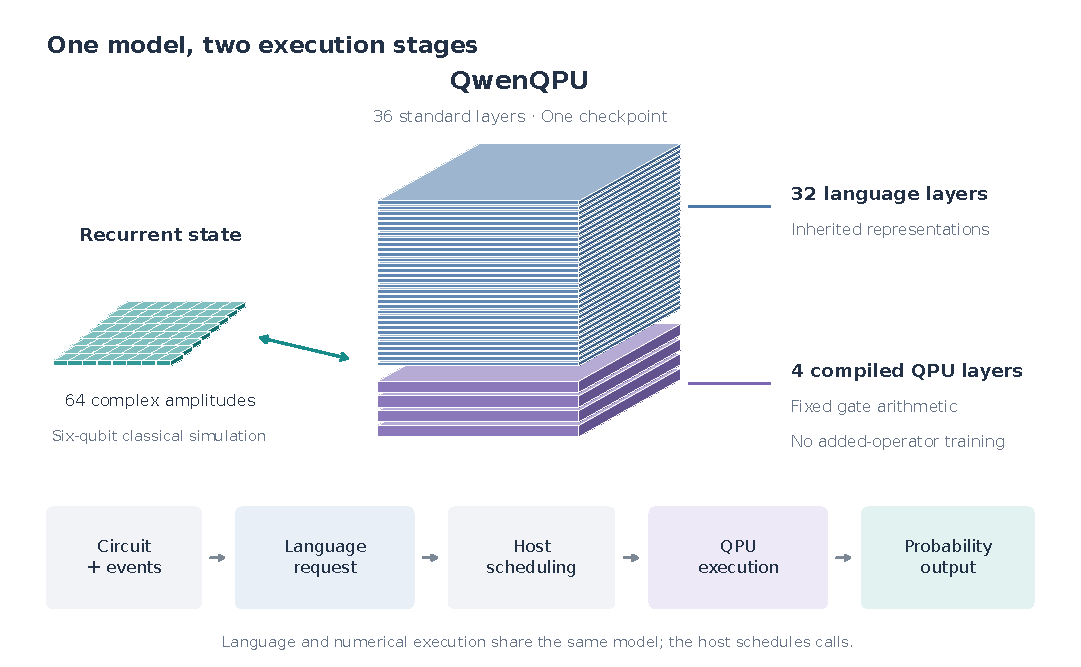
\includegraphics[width=\linewidth]{figures/figure1.pdf}
\caption{\textbf{Language interface and quantum circuit execution within one model.} The three-dimensional stack represents 32 inherited language layers and four fixed-weight QPU layers; in the actual forward order, the QPU layers precede the language layers. Recurrent state stores the 64 complex amplitudes associated with a six-qubit capacity. The lower panel connects circuit and event inputs, language requests, host scheduling, model-internal execution, and probability outputs. The host handles parsing, instruction loading, scheduling, and digit decoding; standard model layers perform amplitude updates and probability arithmetic. The three-dimensional structure is an architectural schematic of state-vector simulation on classical hardware.}
\label{fig:1}
\end{figure}

\section{Model construction and execution}

QwenQPU has two parameter sources: language layers inherited from a pretrained checkpoint and QPU layers analytically constructed from gate coefficients, address logic, digit encoding, and readout rules. The construction procedure maps these rules to projections and recurrent updates in standard layers and assembles them with the language layers; the added execution capability uses no optimizer or additional training data \cite{ref22}. Across repeated forward calls, the four QPU layers jointly implement storage, computation, and output, with roles selected by the gate-execution or probability-query phase (Table 2). We describe state encoding, shared arithmetic, and readout error conditions in turn.

\begin{table}[!htbp]
\centering
\small
\renewcommand{\arraystretch}{1.16}
\caption{\textbf{Main roles of the four QPU layers in gate execution and probability readout.} Layers are numbered from 1. The protocol phase selects which arithmetic units are active within a layer. The table describes the probability-execution path used in this study.}
\label{tab:2}
\begin{tabular}{@{}>{\raggedright\arraybackslash}p{\dimexpr 0.130\linewidth-2\tabcolsep\relax}>{\raggedright\arraybackslash}p{\dimexpr 0.510\linewidth-2\tabcolsep\relax}>{\raggedright\arraybackslash}p{\dimexpr 0.360\linewidth-2\tabcolsep\relax}@{}}
\toprule
\textbf{Layer} & \textbf{State or arithmetic role} & \textbf{Quantities passed to subsequent steps} \\
\midrule
QPU layer 1 & Gated DeltaNet maintains amplitude RAM, instruction ROM, control state, and accumulators. The MLP decodes reads and performs shared gate arithmetic; correction queries decode event mass E and total mass T. & Candidate updated amplitude digits, control values, real and imaginary components, accumulator values \\[2pt]
QPU layer 2 & Converts amplitude digits and control values to Gray codes, forms Born terms from real and imaginary components, and checks control conditions. Correction queries compute E(2\ensuremath{-}T). & Digit and control codes, Born terms, corrected event probability \\[2pt]
QPU layer 3 & Combines Born terms with the accumulator to form probability-digit candidates, or forms candidates from the corrected probability; applies control and query validity constraints. & High- and low-order probability-digit candidates and output constraints \\[2pt]
QPU layer 4 & Converts probability-digit candidates to Gray codes and works with the standard output head to produce digit tokens. & Decodable probability digits, fed back or returned according to the protocol \\[2pt]
\bottomrule
\end{tabular}
\end{table}

These roles follow the fixed-version \href{https://github.com/xi-zhao/QwenQPU/blob/caae45327b46458163d0840a4c1466e5575a7b4f/research/standard_layers/compact_checkpoint.py}{four-layer construction code} and \href{https://github.com/xi-zhao/QwenQPU/blob/caae45327b46458163d0840a4c1466e5575a7b4f/research/standard_layers/experiments/compact_normalized_readout.py}{readout-correction implementation}. Gate execution and probability queries reuse these layers across multiple forward calls and digit-feedback steps; a depth of four layers does not imply that four calls execute an entire circuit.

\subsection{Addressable amplitudes in recurrent state}

Work on linear attention and fast weights establishes the role of recurrent matrices as key--value memory \cite{ref11}, \cite{ref12}. We use Gated DeltaNet to combine state retention and directed writes in recurrent updates \cite{ref13}. An idealized single-head matrix update illustrates this storage role. With state matrix S, key k, and value v, the update can be written as

\begin{equation}
\widetilde S_t=\alpha_t S_{t-1},\qquad
S_t=\widetilde S_t+\beta_t k_t\bigl(v_t^{\mathsf T}-k_t^{\mathsf T}\widetilde S_t\bigr).
\end{equation}

With retention and overwrite settings for the state gate and write strength, one-hot keys address updates to individual storage rows. The compiler uses this mechanism to organize amplitude memory, instruction ROM, the program counter, and accumulators. Replicated storage ports provide the multiple reads required by arithmetic. A quantum state contains 2\textsuperscript{n} complex amplitudes, and each real or imaginary component is represented by two base-4096 digits:

\begin{equation}
r=\frac{4096d_{\mathrm{hi}}+d_{\mathrm{lo}}}{2^{22}}-1,
\qquad d_{\mathrm{hi}},d_{\mathrm{lo}}\in\{0,\ldots,4095\}.
\end{equation}

The resulting numerical grid spacing is 2\textsuperscript{-22}. Digit tokens carry the high- and low-order digits, and the digits emitted by gate operations are fed back into recurrent state to complete the next storage update. Double buffering separates a gate's output from its input state. Arithmetic is reused across addresses, so a separate set of gate-computation rules is not required for each amplitude address.

\subsection{Gate operations through shared arithmetic}

The gate compiler maps H, X, T, and CNOT to address selection and a small set of shared arithmetic forms. For a pair of amplitudes whose target bit is 0 or 1, H computes the normalized sum and difference. T multiplies an amplitude with target bit 1 by exp(i\ensuremath{\pi}/4), which reduces to sums and differences of its real and imaginary components:

\begin{equation}
H:\quad (a_0,a_1)\mapsto\left(\frac{a_0+a_1}{\sqrt2},\frac{a_0-a_1}{\sqrt2}\right),\qquad
T:\quad a+ib\mapsto\frac{a-b}{\sqrt2}+i\frac{a+b}{\sqrt2}.
\end{equation}

X selects source amplitudes by flipping the target address bit; CNOT applies this permutation conditionally on the control bit. The SwiGLU feedforward structure includes an elementwise product of an activated branch and a linear branch \cite{ref23}. We set its projections to analytically specified coefficients and reuse the same arithmetic across gates, addresses, and digit phases; initialization uses the corresponding constant form. The compiler also constructs control tokens, program counting, and stopping conditions, allowing gate sequences to advance through model outputs and feedback \cite{ref22}.

H, T, and CNOT provide universal approximation in the ideal gate-sequence model \cite{ref24}. The scope of the present implementation and experiments is jointly determined by six-qubit storage, the evaluated gate counts, and finite-precision conditions.

\subsection{Born readout and normalization correction}

For each basis state, the execution layers compute the sum of the squared real and imaginary components and accumulate it within the model according to an event mask. Let E denote event mass and T total mass. Because finite precision can cause T to deviate from 1, readout uses the following correction near unit norm:

\begin{equation}
\widehat p=E(2-T),\qquad |T-1|\leq 5\times10^{-4}.
\end{equation}

The multiplication is implemented through SwiGLU's multiplicative structure; the identity SiLU(z)\ensuremath{-}SiLU(\ensuremath{-}z)=z provides a basis for constructing the required linear factor. For T\textgreater0 and 0\ensuremath{\leq}E\ensuremath{\leq}T, the difference between the corrected value and the normalized ratio satisfies

\begin{equation}
\left|\frac ET-E(2-T)\right|=\frac E T(T-1)^2\leq 2.5\times10^{-7}.
\end{equation}

This bound applies only to the normalization approximation. The complete output also includes errors from amplitude evolution, digit quantization, and floating-point arithmetic, so final probabilities are evaluated against an independent state-vector calculation. The host checks the stated norm range and transports digits; event arithmetic and the correction are performed in the fixed layers.

\subsection{Execution protocol and host interface}

We define model-internal execution operationally: model parameters and standard forward operators implement amplitude updates, Born probabilities, and event summation. The host parses gate strings and event indices, loads instructions, builds query masks, schedules calls, selects output tokens, and decodes the final digits. It does not use an external state-vector simulator to generate execution answers. Qiskit and NumPy provide independent validation. The benchmark uses native function-call syntax: the function name provides a scheduling entry point backed by the QPU layers of the same model \cite{ref25}.

\begin{figure}[!htbp]
\centering
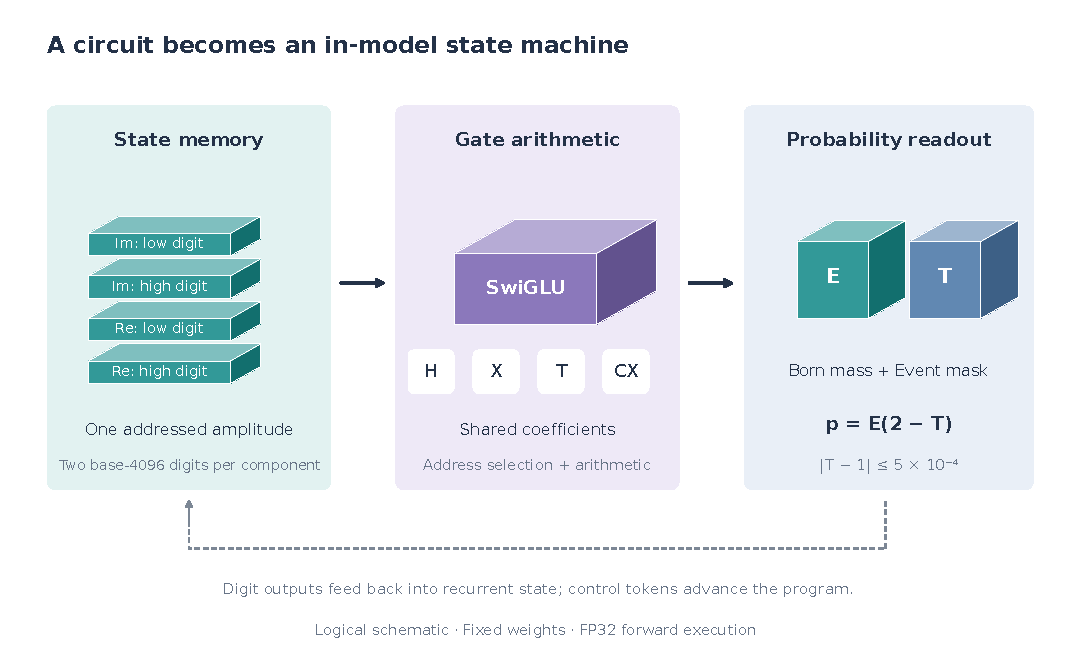
\includegraphics[width=\linewidth]{figures/figure2.pdf}
\caption{\textbf{Model-internal execution from amplitude digits to measurement probabilities.} The real and imaginary parts of each complex amplitude are each encoded by two base-4096 digits; the slabs represent digit components. Fixed SwiGLU projections and address selection implement H, X, T, and CNOT (CX), with output digits fed back to recurrent state. Readout accumulates event mass E and total mass T and applies \(\widehat{p}\)=E(2\ensuremath{-}T) when \textbar T\ensuremath{-}1\textbar{}\ensuremath{\leq}5\ensuremath{\times}10\textsuperscript{-4}. The schematic groups functions into storage, arithmetic, and readout; these blocks do not correspond one-to-one to separate physical devices or model layers. The added operator weights are analytically constructed.}
\label{fig:2}
\end{figure}

\section{Evaluation}

\subsection{Frozen tasks and independent references}

The primary benchmark contains 36 non-Clifford tasks: four circuits for each of the nine combinations of 3, 4, or 6 logical qubits and 12, 18, or 24 sequential gates. An additional 12 Clifford control tasks contain four 18-gate circuits at each register size. Every task starts from the all-zero state. Event A specifies one bit and event B specifies two bits, with the remaining bits marginalized \cite{ref25}.

Before model inference, candidate circuits are screened using physical criteria: a connected interaction graph, entanglement in the final state, and event probabilities in {[}0.025,0.975{]}. Non-Clifford tasks additionally require at least one event probability to be more than 0.001 from every multiple of 1/16. Screening does not use model answers. Tasks and the evaluation protocol are frozen before inference. Independent NumPy and Qiskit Statevector implementations \cite{ref26} agree across all tasks and two additional interface probes, with a maximum probability difference of 6.66\ensuremath{\times}10\textsuperscript{-16} \cite{ref25}. The probes are excluded from the 48 main tasks.

\subsection{Paired conditions and budgets}

Both conditions use the same assembled checkpoint and tasks. The baseline disables the quantum-execution entry point and obtains probabilities directly from the language component. QwenQPU receives a native function definition and returns numerical answers from its own QPU after submitting the circuit and events. The shared system prompt requires immediate function use when available and self-contained calculation otherwise. This paired design holds language weights fixed while changing the availability of execution and its interface. The term ``Qwen baseline'' denotes this disabled condition throughout. The experiment does not include a condition in which the same language model calls an external simulator.

Each condition has a total prediction budget of 16,384. Language tokens, function arguments, and every native QPU forward prediction count toward this ceiling, which is not reset after a function call; host-supplied control tokens are recorded separately. The two conditions share a generation seed for each task. Task order is shuffled with a fixed seed, and the condition executed first is alternated.

Language decoding uses the native non-thinking template with temperature=1, top-p=0.95, top-k=20, presence penalty=1.5, and repetition penalty=1. The time limit is 3,600 seconds per condition, and completed failures are not regenerated. The experiment is a single-seed paired evaluation on a fixed task set.

\subsection{Success criteria}

Numerical success requires both event probabilities, A and B, to differ from the Qiskit complex128 reference by no more than 5\ensuremath{\times}10\textsuperscript{-5}. QwenQPU must also submit the same event sets as the task, and the submitted circuit must produce a final-state infidelity below 10\textsuperscript{-10} for the specified initial state. This circuit criterion verifies agreement for that initial state; it does not require operator equivalence on all possible inputs.

Formatting errors, contradictory answers, missing probabilities, truncation, and timeouts remain in the denominator. Identical repeated JSON answers may be consolidated; conflicting answers count as failures. The statistical unit is the task, and the two events within a task are not treated as independent samples. We report Wilson intervals for success rates \cite{ref27}, two-sided exact conditional McNemar tests \cite{ref28}, \cite{ref29}, and conservative intervals for paired differences based on Clopper--Pearson intervals \cite{ref30}. Appendix B specifies the calculations.

\subsection{Implementation and measurement}

Evaluation uses an NVIDIA A100 80 GB GPU, PyTorch 2.6.0+cu124, and Transformers 5.19.0, with numerical execution in FP32 and TF32 disabled. Timing includes language decoding, native execution, and progress input/output, is measured after CUDA synchronization, and excludes model loading. Peak allocated GPU memory is 38.56 GB for the baseline and 38.40 GB for QwenQPU. ``Equal budget'' refers to the same prediction-count ceiling, not to equal realized prediction counts, FLOPs, or runtime.

\section{Model capabilities and execution cost}

\subsection{Internal execution satisfies all criteria on 48 frozen tasks}

QwenQPU meets the numerical and request-fidelity criteria on all 48 frozen tasks, compared with four for the baseline, a difference of 91.67 percentage points. All 44 discordant pairs favor QwenQPU; both conditions are correct on the remaining four tasks. The non-Clifford primary endpoint improves from 2/36 to 36/36 (Table 3), showing that the gain extends to the evaluated circuits containing T gates.

\begin{table}[!htbp]
\centering
\small
\renewcommand{\arraystretch}{1.16}
\caption{\textbf{Paired results on the frozen task set.} Success requires both event probabilities to pass. Non-Clifford and Clifford rows form disjoint subsets of the benchmark.}
\label{tab:3}
\begin{tabular}{@{}>{\raggedright\arraybackslash}p{\dimexpr 0.400\linewidth-2\tabcolsep\relax}>{\raggedright\arraybackslash}p{\dimexpr 0.100\linewidth-2\tabcolsep\relax}>{\raggedright\arraybackslash}p{\dimexpr 0.250\linewidth-2\tabcolsep\relax}>{\raggedright\arraybackslash}p{\dimexpr 0.250\linewidth-2\tabcolsep\relax}@{}}
\toprule
\textbf{Task family} & \textbf{Tasks} & \textbf{Qwen baseline} & \textbf{QwenQPU} \\
\midrule
Non-Clifford primary endpoint & 36 & 2/36, 5.6\% & 36/36, 100\% \\[2pt]
Clifford controls & 12 & 2/12, 16.7\% & 12/12, 100\% \\[2pt]
All tasks & 48 & 4/48, 8.3\% & 48/48, 100\% \\[2pt]
\bottomrule
\end{tabular}
\end{table}

The conservative exact 95\% interval for the overall paired improvement is 69.50--98.12 percentage points, with a two-sided exact McNemar p=1.1369\ensuremath{\times}10\textsuperscript{-13}. The improvement on the non-Clifford primary endpoint is 94.44 percentage points, with p=1.1642\ensuremath{\times}10\textsuperscript{-10}. Appendix B provides success-rate intervals and further statistical details. These statistics describe the single-seed paired results for the frozen task family; inference across task distributions or seeds requires corresponding replication.

\begin{figure}[!htbp]
\centering
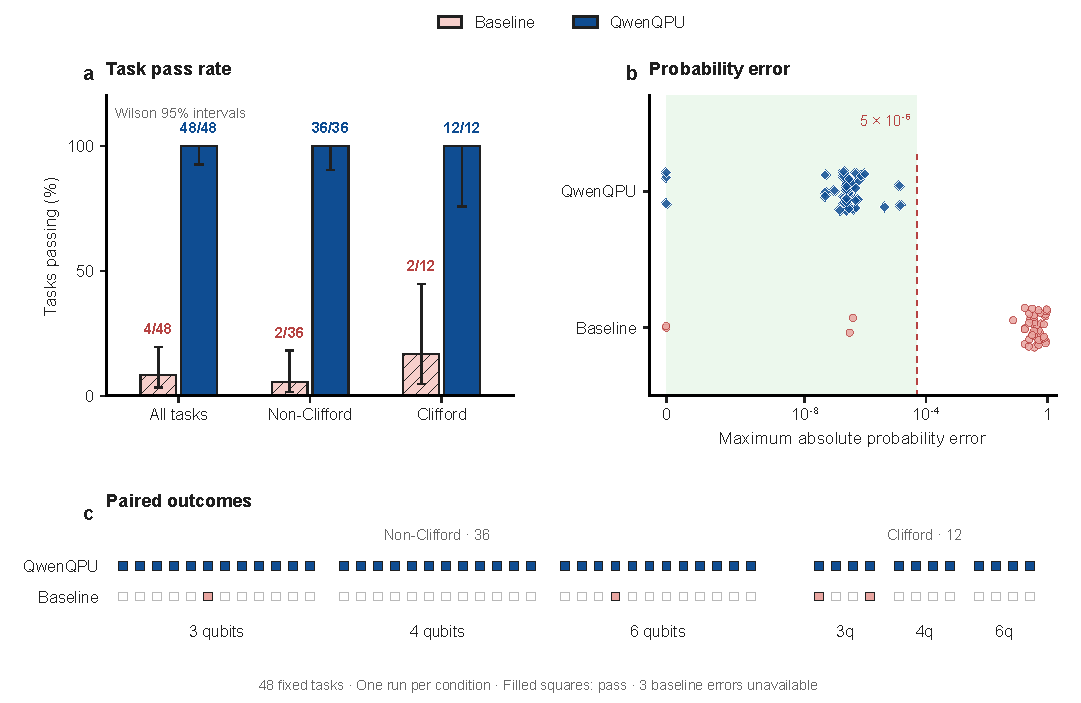
\includegraphics[width=\linewidth]{figures/figure3.pdf}
\caption{\textbf{Paired results for 48 frozen tasks.} a, Grouped bars show success rates from a zero baseline, labeled with exact successful-task counts and denominators; black intervals are Wilson 95\% intervals. ``All'' combines 36 non-Clifford and 12 Clifford tasks. b, Each point shows the larger absolute error of the two event probabilities in one run: 48 QwenQPU points and 45 valid numerical baseline outputs. The other three baseline failures have no valid numerical error but remain in the success-rate denominator. The symmetric-log horizontal axis retains a linear region near zero (threshold 10\textsuperscript{-12}); the red dashed line marks the 5\ensuremath{\times}10\textsuperscript{-5} criterion, and the pale-green region lies within it. c, Each column pairs the two conditions for one task; filled squares indicate success and open squares failure. Conditions share language weights and a ceiling of 16,384 predictions, with one run per task per condition. All 96 records are retained: 44 failures become successes and four existing successes are preserved. Vertical jitter in the error scatter reduces overlap without changing error values. Data comprise all r5 records from the fixed version \cite{ref25}.}
\label{fig:3}
\end{figure}

By logical register size, the baseline succeeds on 3/16, 0/16, and 1/16 tasks at 3, 4, and 6 qubits, respectively, whereas QwenQPU succeeds on 16/16 at each size. In the non-Clifford subsets with 12, 18, and 24 gates, the baseline succeeds on 1/12, 1/12, and 0/12, respectively, versus 12/12 for QwenQPU in each subset. These strata describe different logical task sizes within the same six-qubit storage model; they do not test scalability under an increase in model storage capacity.

\subsection{Probability errors and representative circuits meet numerical requirements}

Across the 48 tasks, QwenQPU's maximum absolute probability error is 1.4209657\ensuremath{\times}10\textsuperscript{-5}, below the prespecified threshold of 5\ensuremath{\times}10\textsuperscript{-5}, and every request reaches numerical completion within the prediction budget. The baseline's 44 failures comprise 41 numerical errors, two conflicting answers, and one answer missing the required A/B probabilities; all 48 baseline generations terminate normally with EOS. Baseline failures therefore primarily manifest as probability outputs that do not meet the numerical tolerance. This output classification alone does not identify the internal cause of the errors.

Two complete-model demonstrations test phase interference and joint readout across multiple qubits. H3--T3--H3 converts a phase difference into measurement probabilities, while a six-qubit GHZ circuit tests a CNOT chain and joint-event aggregation. In both demonstrations, the language model first generates a request and the QPU layers of the complete assembled model return the numerical answer. These demonstrations are excluded from the 48 tasks in Table 3 \cite{ref22}.

\begin{table}[!htbp]
\centering
\small
\renewcommand{\arraystretch}{1.16}
\caption{\textbf{Independent demonstrations with the complete model.} Qubit indices start at 0, and both circuits begin in the six-qubit all-zero state.}
\label{tab:4}
\begin{tabular}{@{}>{\raggedright\arraybackslash}p{\dimexpr 0.380\linewidth-2\tabcolsep\relax}>{\raggedright\arraybackslash}p{\dimexpr 0.230\linewidth-2\tabcolsep\relax}>{\raggedright\arraybackslash}p{\dimexpr 0.230\linewidth-2\tabcolsep\relax}>{\raggedright\arraybackslash}p{\dimexpr 0.160\linewidth-2\tabcolsep\relax}@{}}
\toprule
\textbf{Circuit and event} & \textbf{QwenQPU} & \textbf{Reference probability} & \textbf{Absolute error} \\
\midrule
H3--T3--H3, q3=1 & 0.1464464664 & 0.1464466094 & 1.43\ensuremath{\times}10\textsuperscript{-7} \\[2pt]
H3--T3--H3, all zeros & 0.8535535336 & 0.8535533906 & 1.43\ensuremath{\times}10\textsuperscript{-7} \\[2pt]
H0 followed by CNOT chain 0\ensuremath{\rightarrow}1\ensuremath{\rightarrow}2\ensuremath{\rightarrow}3\ensuremath{\rightarrow}4\ensuremath{\rightarrow}5, all zeros & 0.5 & 0.5 & 1.11\ensuremath{\times}10\textsuperscript{-16} \\[2pt]
Same GHZ circuit, all ones & 0.5 & 0.5 & 1.11\ensuremath{\times}10\textsuperscript{-16} \\[2pt]
\bottomrule
\end{tabular}
\end{table}

\begin{figure}[!htbp]
\centering
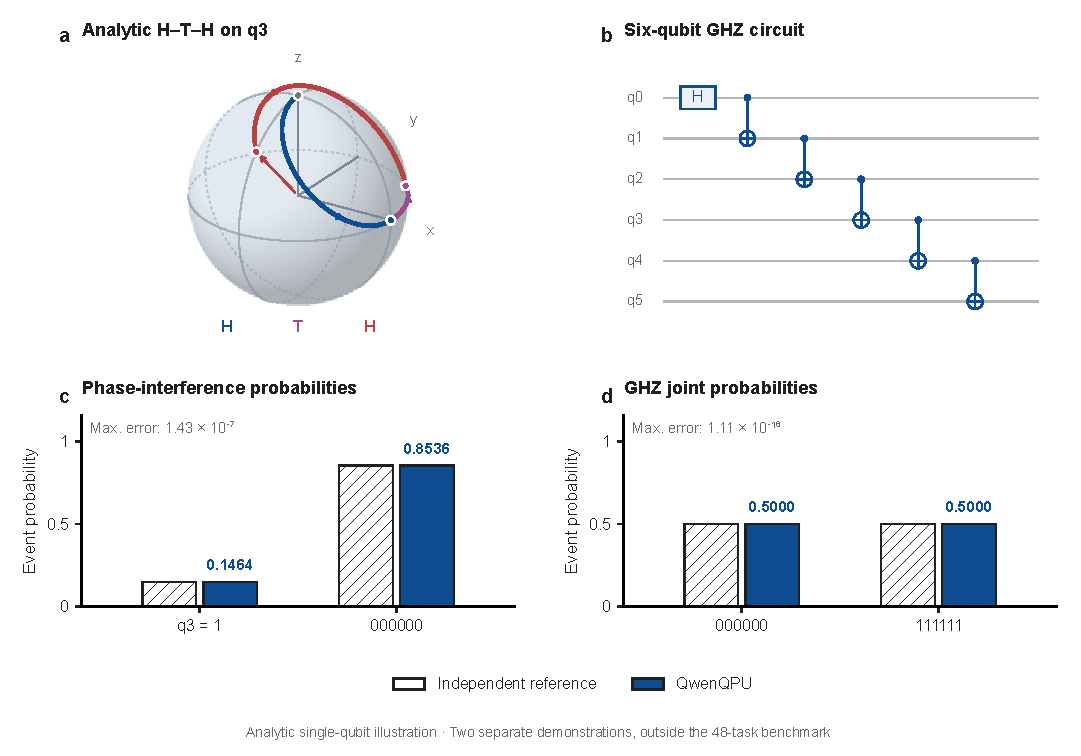
\includegraphics[width=\linewidth]{figures/figure4.pdf}
\caption{\textbf{Phase interference and six-qubit joint probabilities.} a, Analytical Bloch-sphere schematic of H--T--H on active qubit q3, initially in \(\lvert0\rangle\). Surface shading represents geometric illumination and arcs represent analytical rotations, not measured internal model trajectories. b, H0 and successive CNOT gates form a six-qubit GHZ circuit. c,d, Hatched open bars show independent reference probabilities and dark-blue bars show saved complete-model outputs, all on a 0--1 probability scale. Blue labels report rounded model outputs. Maximum absolute errors are 1.43\ensuremath{\times}10\textsuperscript{-7} and 1.11\ensuremath{\times}10\textsuperscript{-16}, respectively. Each circuit starts in the six-qubit all-zero state and has one complete-model demonstration; neither is included in the 48 tasks in Figure 3, and no repeated-measurement error bars are shown. The GHZ panel tests computational-basis joint probabilities of the ideal simulated circuit.}
\label{fig:4}
\end{figure}

These demonstrations check output agreement for phase-gate and controlled-gate composition and event aggregation in two interpretable circuits. The GHZ result concerns only computational-basis joint probabilities; independent certification of coherence or entanglement requires additional observables.

\subsection{Normalization correction reduces readout error on a saved final state}

To examine how finite-precision norm drift affects probability readout, we compare uncorrected and corrected outputs from the same saved final state. For the state saved after a six-qubit, 1,000-gate run, the uncorrected probability error for the event containing all outcomes is approximately 1.21\ensuremath{\times}10\textsuperscript{-4}. After applying the correction in Section 3.3, the maximum error across nine reference comparisons is 1.072\ensuremath{\times}10\textsuperscript{-5}. This result supports the readout correction for that saved state near unit norm. Because the full 1,000-gate circuit was not rerun with all corrections incorporated, this is not an end-to-end validation of long-circuit accuracy. Task-success results in Table 3 come from independent complete runs of the 12-, 18-, and 24-gate circuits.

\subsection{Execution cost is explicitly determined by gate count}

Under the current protocol with six-qubit capacity and two measurement events, the number of QPU predictions is a deterministic function of the sequential gate count:

\begin{equation}
N_{\mathrm{QPU}}(G)=2063+514G.
\end{equation}

Tasks with 12, 18, and 24 gates require 8,231, 11,315, and 14,399 QPU predictions, respectively, totaling 543,120 across the 48 tasks. Every task agrees with this expression. The relation measures cost under a fixed execution protocol; a change in qubit capacity, the number of readout events, or scheduling rules requires the corresponding cost to be recalculated.

\begin{table}[!htbp]
\centering
\small
\renewcommand{\arraystretch}{1.16}
\caption{\textbf{Actual resource use for 48 paired tasks.} Each condition includes all 48 runs, including successes and failures. Amortized time per correct task is total runtime divided by the number of correct tasks, not the mean latency of successful runs.}
\label{tab:5}
\begin{tabular}{@{}>{\raggedright\arraybackslash}p{\dimexpr 0.520\linewidth-2\tabcolsep\relax}>{\raggedright\arraybackslash}p{\dimexpr 0.240\linewidth-2\tabcolsep\relax}>{\raggedright\arraybackslash}p{\dimexpr 0.240\linewidth-2\tabcolsep\relax}@{}}
\toprule
\textbf{Metric} & \textbf{Qwen baseline} & \textbf{QwenQPU} \\
\midrule
Total language predictions & 238,639 & 8,007 \\[2pt]
Total QPU predictions & 0 & 543,120 \\[2pt]
Combined predictions & 238,639 & 551,127 \\[2pt]
Total end-to-end runtime, s & 11,138.90 & 24,974.09 \\[2pt]
Median task runtime, s & 1.87 & 524.20 \\[2pt]
Amortized time per correct task, s & 2,784.72 & 520.29 \\[2pt]
\bottomrule
\end{tabular}
\end{table}

\begin{figure}[!htbp]
\centering
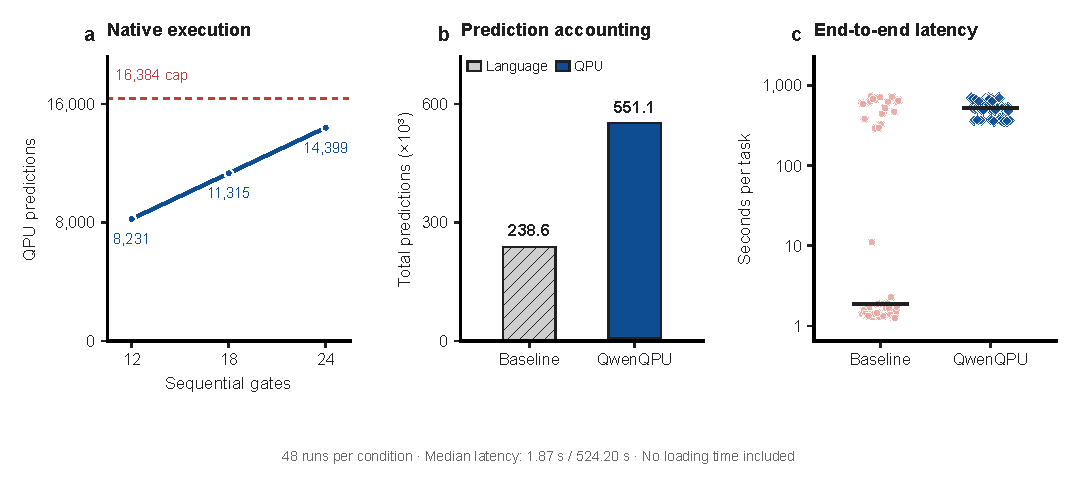
\includegraphics[width=\linewidth]{figures/figure5.pdf}
\caption{\textbf{Execution cost and measured runtime.} a, The fixed six-qubit, two-event protocol satisfies \(N_{\mathrm{QPU}}=2{,}063+514G\); the three points correspond to 12, 18, and 24 gates. The red dashed line marks the shared total ceiling of 16,384 predictions, including language and QPU predictions. b, Total language and native QPU predictions across all 48 tasks, retaining successful and failed runs: 551,127 for QwenQPU and 238,639 for the baseline. Bar values are in thousands. c, Each point is the end-to-end runtime of one task, with 48 points per condition. The vertical axis is logarithmic, and black horizontal lines show medians of 1.87 s and 524.20 s. Timing excludes model loading and includes language generation, native execution, and progress input/output. Under these conditions, the capability gain comes with more total predictions and longer total runtime.}
\label{fig:5}
\end{figure}

The accuracy gain comes with greater actual execution expenditure: QwenQPU uses 551,127 predictions, approximately 2.31 times the baseline's 238,639. Total runtime rises from 11,138.90 s to 24,974.09 s, and median task runtime rises from 1.87 s to 524.20 s (Table 5 and Figure 5). Language predictions decrease to 8,007, while numerical computation is carried by 543,120 QPU predictions. Amortized time, calculated by dividing total runtime by the number of correct tasks, decreases from 2,784.72 s to 520.29 s. This quantity reflects the rate of producing correct results on the current task set; it does not establish faster individual responses or greater efficiency than an external simulator.

\section{Discussion}

QwenQPU shows that analytical numerical rules can form an executable model together with a pretrained language interface when connected through explicit state representations and a readout protocol. Addressable recurrent state associates each amplitude component with an inspectable storage location. Shared arithmetic lets the same projections implement gate operations at different addresses, and the readout correction connects finite-precision state to final probabilities. Together, these components establish a correspondence between internal mathematical variables and task outputs that can be tested through independent references and complete execution records.

Building on program-to-weight construction and recurrent-memory research \cite{ref5}, \cite{ref6}, \cite{ref13}, this work extends validation to successive complex-state evolution and event-probability aggregation. A central design lesson is that execution rules, numerical encoding, and error conditions must be developed together. Fixed gate rules do not automatically guarantee numerical accuracy for arbitrarily long circuits. The saved-state correction result further motivates separate evaluation of state-evolution errors and probability-aggregation errors.

The paired experiment establishes the contribution of access to numerical execution on the evaluated tasks, but does not distinguish the benefit of having a reliable executor from the benefit of placing that executor inside the model. Assessing execution location itself requires a matched condition in which the same language model calls an external simulator through the same request protocol. Tasks, scoring, and resource accounting should be held consistent before comparing accuracy, latency, and deployment overhead. This is a direct next comparison for evaluating the value of model-internal execution.

The evidence covers six-qubit simulation capacity, the H/X/T/CNOT gate set, the all-zero initial state, ideal terminal measurement, and a fixed task family. Three- and four-qubit tasks use the same six-qubit storage, so the results do not establish cost scaling under increased capacity; explicit state-vector storage still grows as 2\textsuperscript{n}. Each condition has one generation, leaving broader task distributions, multiple initial states, and stability across seeds to be evaluated. QPU here denotes a state-vector execution component on classical hardware; the study provides no evidence of physical quantum speedup.

Within these bounds, QwenQPU provides a concrete system for studying numerical execution inside language models. Capabilities can be traced to known rules, errors can be separated into state and readout contributions, and execution expenditure can be counted under a specified protocol. Capacity extensions and implementation improvements can use these verifiable quantities to examine the relationship between accuracy, reliability, and resource cost.

\section{Conclusion}

QwenQPU implements addressable complex amplitudes, shared quantum-gate arithmetic, and probability readout in four fixed-weight layers, combining them with pretrained language layers for circuit interpretation and numerical execution. On 48 frozen paired tasks, enabling execution increases the number of successful tasks from four to 48, with a maximum probability error of 1.42\ensuremath{\times}10\textsuperscript{-5}. Prediction counts increase linearly with gate count under the fixed protocol, and the model consumes more total predictions and runtime than the baseline. Within six-qubit capacity and the evaluated circuit range, this work establishes an implementation path from analytical numerical rules through standard model forward computation to verifiable task results, providing a reproducible basis for studying the accuracy and cost of model-internal execution.

\section*{AI assistance}

OpenAI ChatGPT/Codex was used to assist with manuscript drafting, English translation and language editing, preparation of figure-generation code, and LaTeX typesetting. Responsibility for the scientific claims, data, and references rests with the human authors.

\section*{Code and data availability}

The compiler, model-assembly code, task interface, frozen task list, per-condition result extracts, and scoring code are available in the \href{https://github.com/xi-zhao/QwenQPU/tree/caae45327b46458163d0840a4c1466e5575a7b4f}{QwenQPU code repository}. The main experiment uses the standard added-layer implementation in research/standard\_layers, with results in evidence/added-layers. Main tables can be reconstructed from the 96 released condition records; rerunning model generation requires the corresponding checkpoints and runtime environment. The experiment is identified jointly by a fixed code commit, the upstream language-checkpoint revision, and hashes of the four-layer QPU prefix, as specified in Appendix A.

The model distribution entry point is \href{https://huggingface.co/xi-zhao/QwenQPU}{xi-zhao/QwenQPU}. The fixed-version experiment manifest records a model assembled and executed in memory. Reproduction should verify its components and weight hashes rather than substitute the distribution repository's mutable main branch for the experimental model identity. Establishing that a complete serialized checkpoint matches this identity requires a corresponding release manifest and readback-validation records. Sources of inherited weights, construction methods, and code components are documented in the \href{https://github.com/xi-zhao/QwenQPU/blob/caae45327b46458163d0840a4c1466e5575a7b4f/docs/LICENSES.md}{attribution and licensing statement}.

\begin{thebibliography}{30}

\bibitem{ref1}
Schick T, Dwivedi-Yu J, Dessì R, et al.~Toolformer: Language Models Can Teach Themselves to Use Tools. Advances in Neural Information Processing Systems, 36, 2023. \href{https://proceedings.neurips.cc/paper_files/paper/2023/hash/d842425e4bf79ba039352da0f658a906-Abstract-Conference.html}{Publication record}. \href{https://arxiv.org/abs/2302.04761}{arXiv:2302.04761}.

\bibitem{ref2}
Gao L, Madaan A, Zhou S, et al.~PAL: Program-aided Language Models. Proceedings of ICML, PMLR 202:10764--10799, 2023. \href{https://proceedings.mlr.press/v202/gao23f.html}{Article}.

\bibitem{ref3}
Chen W, Ma X, Wang X, Cohen W W. Program of Thoughts Prompting: Disentangling Computation from Reasoning for Numerical Reasoning Tasks. Transactions on Machine Learning Research, 2023. \href{https://arxiv.org/abs/2211.12588}{Article}.

\bibitem{ref4}
Yao S, Zhao J, Yu D, et al.~ReAct: Synergizing Reasoning and Acting in Language Models. ICLR, 2023. \href{https://arxiv.org/abs/2210.03629}{Article}.

\bibitem{ref5}
Weiss G, Goldberg Y, Yahav E. Thinking Like Transformers. Proceedings of ICML, PMLR 139:11080--11090, 2021. \href{https://proceedings.mlr.press/v139/weiss21a.html}{Paper and publication record}.

\bibitem{ref6}
Lindner D, Kramár J, Farquhar S, Rahtz M, McGrath T, Mikulik V. Tracr: Compiled Transformers as a Laboratory for Interpretability. Advances in Neural Information Processing Systems, 36, 2023. \href{https://proceedings.neurips.cc/paper_files/paper/2023/hash/771155abaae744e08576f1f3b4b7ac0d-Abstract-Conference.html}{Publication record}. \href{https://arxiv.org/abs/2301.05062}{arXiv:2301.05062}.

\bibitem{ref7}
Pérez J, Barceló P, Marinkovic J. Attention is Turing-Complete. Journal of Machine Learning Research, 22(75):1--35, 2021. \href{https://jmlr.org/papers/v22/20-302.html}{Article}.

\bibitem{ref8}
Agrawal D. Qwenputer: a fully functioning, deterministic RISC-V CPU inside Qwen3.5. 22 October 2026. Technical blog post. Accessed 11 November 2026. \href{https://divagr.com/blog/qwenputer}{Project report}.

\bibitem{ref9}
Graves A, Wayne G, Danihelka I. Neural Turing Machines. arXiv:1410.5401, 2014. \href{https://arxiv.org/abs/1410.5401}{Article}.

\bibitem{ref10}
Graves A, Wayne G, Reynolds M, et al.~Hybrid computing using a neural network with dynamic external memory. Nature, 538(7626):471--476, 2016. DOI: 10.1038/nature20101. \href{https://www.nature.com/articles/nature20101}{Article}.

\bibitem{ref11}
Katharopoulos A, Vyas A, Pappas N, Fleuret F. Transformers are RNNs: Fast Autoregressive Transformers with Linear Attention. Proceedings of ICML, PMLR 119:5156--5165, 2020. \href{https://proceedings.mlr.press/v119/katharopoulos20a.html}{Article}.

\bibitem{ref12}
Schlag I, Irie K, Schmidhuber J. Linear Transformers Are Secretly Fast Weight Programmers. Proceedings of ICML, PMLR 139:9355--9366, 2021. \href{https://proceedings.mlr.press/v139/schlag21a.html}{Article}.

\bibitem{ref13}
Yang S, Kautz J, Hatamizadeh A. Gated Delta Networks: Improving Mamba2 with Delta Rule. ICLR, 2025. \href{https://arxiv.org/abs/2412.06464}{arXiv:2412.06464}.

\bibitem{ref14}
Barenco A, Bennett C H, Cleve R, et al.~Elementary gates for quantum computation. Physical Review A, 52:3457--3467, 1995. DOI: 10.1103/PhysRevA.52.3457. \href{https://arxiv.org/abs/quant-ph/9503016}{Article}.

\bibitem{ref15}
Aaronson S, Gottesman D. Improved Simulation of Stabilizer Circuits. Physical Review A, 70:052328, 2004. DOI: 10.1103/PhysRevA.70.052328. \href{https://arxiv.org/abs/quant-ph/0406196}{Article}.

\bibitem{ref16}
Vidal G. Efficient classical simulation of slightly entangled quantum computations. Physical Review Letters, 91:147902, 2003. DOI: 10.1103/PhysRevLett.91.147902. \href{https://arxiv.org/abs/quant-ph/0301063}{Article}.

\bibitem{ref17}
Markov I L, Shi Y. Simulating quantum computation by contracting tensor networks. SIAM Journal on Computing, 38(3):963--981, 2008. DOI: 10.1137/050644756. \href{https://arxiv.org/abs/quant-ph/0511069}{Article}.

\bibitem{ref18}
Jones T, Brown A, Bush I, Benjamin S C. QuEST and High Performance Simulation of Quantum Computers. Scientific Reports, 9:10736, 2019. DOI: 10.1038/s41598-019-47174-9. \href{https://www.nature.com/articles/s41598-019-47174-9}{Article}.

\bibitem{ref19}
Suzuki Y, Kawase Y, Masumura Y, et al.~Qulacs: a fast and versatile quantum circuit simulator for research purpose. Quantum, 5:559, 2021. DOI: 10.22331/q-2021-10-06-559. \href{https://quantum-journal.org/papers/q-2021-10-06-559/}{Article}.

\bibitem{ref20}
Carleo G, Troyer M. Solving the Quantum Many-Body Problem with Artificial Neural Networks. Science, 355:602--606, 2017. DOI: 10.1126/science.aag2302. \href{https://arxiv.org/abs/1606.02318}{Article}.

\bibitem{ref21}
Qwen Team. Qwen3.5-4B model card. 2026. Accessed 11 November 2026. \href{https://huggingface.co/Qwen/Qwen3.5-4B}{Official model card}.

\bibitem{ref22}
QwenQPU contributors. QPU in standard Qwen layers. Project documentation, commit \texttt{caae4532\allowbreak{}7b464581\allowbreak{}63d0840a\allowbreak{}4c1466e5\allowbreak{}575a7b4f}, 2026. \href{https://github.com/xi-zhao/QwenQPU/blob/caae45327b46458163d0840a4c1466e5575a7b4f/docs/ADDED_LAYERS.md}{Implementation and demonstrations}.

\bibitem{ref23}
Shazeer N. GLU Variants Improve Transformer. arXiv:2002.05202, 2020. \href{https://arxiv.org/abs/2002.05202}{Article}.

\bibitem{ref24}
Boykin P O, Mor T, Pulver M, Roychowdhury V, Vatan F. On Universal and Fault-Tolerant Quantum Computing. arXiv:quant-ph/9906054, 1999. \href{https://arxiv.org/abs/quant-ph/9906054}{Article}.

\bibitem{ref25}
QwenQPU contributors. Supplied-circuit probability benchmark (r5). Project documentation and data, commit \texttt{caae4532\allowbreak{}7b464581\allowbreak{}63d0840a\allowbreak{}4c1466e5\allowbreak{}575a7b4f}, 2026. \href{https://github.com/xi-zhao/QwenQPU/blob/caae45327b46458163d0840a4c1466e5575a7b4f/docs/BENCHMARK_ADDED_LAYERS.md}{Tasks and evaluation protocol}; \href{https://github.com/xi-zhao/QwenQPU/blob/caae45327b46458163d0840a4c1466e5575a7b4f/evidence/added-layers/r5-plot-data.json}{Per-condition results}; \href{https://github.com/xi-zhao/QwenQPU/blob/caae45327b46458163d0840a4c1466e5575a7b4f/evidence/added-layers/r5-final.json}{Summary statistics}.

\bibitem{ref26}
IBM Quantum. Qiskit Statevector API documentation. Accessed 11 November 2026. \href{https://quantum.cloud.ibm.com/docs/en/api/qiskit/qiskit.quantum_info.Statevector}{Official documentation}.

\bibitem{ref27}
Wilson E B. Probable Inference, the Law of Succession, and Statistical Inference. Journal of the American Statistical Association, 22(158):209--212, 1927. DOI: 10.1080/01621459.1927.10502953. \href{https://www.tandfonline.com/doi/abs/10.1080/01621459.1927.10502953}{Article}.

\bibitem{ref28}
McNemar Q. Note on the sampling error of the difference between correlated proportions or percentages. Psychometrika, 12(2):153--157, 1947. DOI: 10.1007/BF02295996. \href{https://link.springer.com/article/10.1007/BF02295996}{Article}.

\bibitem{ref29}
Fagerland M W, Lydersen S, Laake P. The McNemar test for binary matched-pairs data: mid-p and asymptotic are better than exact conditional. BMC Medical Research Methodology, 13:91, 2013. DOI: 10.1186/1471-2288-13-91. \href{https://link.springer.com/article/10.1186/1471-2288-13-91}{Article}.

\bibitem{ref30}
Clopper C J, Pearson E S. The use of confidence or fiducial limits illustrated in the case of the binomial. Biometrika, 26(4):404--413, 1934. DOI: 10.1093/biomet/26.4.404. \href{https://academic.oup.com/biomet/article-abstract/26/4/404/291538}{Article}.

\end{thebibliography}

\clearpage

\appendix

\setcounter{table}{0}

\renewcommand{\thetable}{A\arabic{table}}

\section{Reproduction settings and versions}

\begin{table}[!htbp]
\centering
\small
\renewcommand{\arraystretch}{1.16}
\caption{Reproduction settings and fixed versions.}
\label{tab:a1}
\begin{tabular}{@{}>{\raggedright\arraybackslash}p{\dimexpr 0.290\linewidth-2\tabcolsep\relax}>{\raggedright\arraybackslash}p{\dimexpr 0.710\linewidth-2\tabcolsep\relax}@{}}
\toprule
\textbf{Item} & \textbf{Setting} \\
\midrule
Language source & Qwen3.5-4B, inherited through a fixed Qwenputer checkpoint \\[2pt]
Upstream checkpoint & divagr1925/Qwen3.5-4B-Qwenputer \\[2pt]
Code commit & \texttt{caae4532\allowbreak{}7b464581\allowbreak{}63d0840a\allowbreak{}4c1466e5\allowbreak{}575a7b4f} \\[2pt]
Upstream revision & \texttt{2d906850\allowbreak{}8f2b680b\allowbreak{}adb7abcd\allowbreak{}ed96fdd1\allowbreak{}07e9ba5d} \\[2pt]
Standard-layer model & 32 language layers and 4 QPU layers \\[2pt]
Numerical mode & FP32; TF32 disabled \\[2pt]
Software & PyTorch 2.6.0+cu124; Transformers 5.19.0 \\[2pt]
Physical compute device & NVIDIA A100 80 GB GPU \\[2pt]
Simulated register capacity & 6 qubits \\[2pt]
Evaluation size & 48 tasks; 96 paired-condition records \\[2pt]
Numerical criterion & Absolute error \ensuremath{\leq}5\ensuremath{\times}10\textsuperscript{-5} for both events \\[2pt]
Request criterion & Matching events; final-state infidelity \textless10\textsuperscript{-10} from the all-zero initial state \\[2pt]
Budget and time limit & 16,384 generated predictions; 3,600 s per condition \\[2pt]
\bottomrule
\end{tabular}
\end{table}

The four-layer QPU prefix consists of two FP32 safetensors files. The hashes below come from the \href{https://github.com/xi-zhao/QwenQPU/blob/caae45327b46458163d0840a4c1466e5575a7b4f/evidence/added-layers/weight-manifest.json}{weight manifest} at the fixed code version. They distinguish the execution prefix from the language source and the complete assembled model; the two prefix files alone do not contain the full language model.

\begin{table}[!htbp]
\centering
\small
\renewcommand{\arraystretch}{1.16}
\caption{QPU prefix files and SHA-256 identities.}
\label{tab:a2}
\begin{tabular}{@{}>{\raggedright\arraybackslash}p{\dimexpr 0.320\linewidth-2\tabcolsep\relax}>{\raggedright\arraybackslash}p{\dimexpr 0.180\linewidth-2\tabcolsep\relax}>{\raggedright\arraybackslash}p{\dimexpr 0.500\linewidth-2\tabcolsep\relax}@{}}
\toprule
\textbf{QPU prefix file} & \textbf{Bytes} & \textbf{SHA-256} \\
\midrule
\texttt{model-\allowbreak{}00001-\allowbreak{}of-\allowbreak{}00002.\allowbreak{}safetensors} & 985,465,312 & \texttt{d92ff7c2\allowbreak{}7df6b4f0\allowbreak{}c3eb9782\allowbreak{}1652a77f\allowbreak{}b38be34b\allowbreak{}72b272ee\allowbreak{}0d8e53bf\allowbreak{}363f6178} \\[2pt]
\texttt{model-\allowbreak{}00002-\allowbreak{}of-\allowbreak{}00002.\allowbreak{}safetensors} & 437,023,752 & \texttt{03a3c8ce\allowbreak{}85ba089a\allowbreak{}4ea17aa8\allowbreak{}8b8324e9\allowbreak{}11d67a2c\allowbreak{}0801cc83\allowbreak{}e5300714\allowbreak{}93d27730} \\[2pt]
\bottomrule
\end{tabular}
\end{table}

The frozen task list has SHA-256 \texttt{b6d892f5\allowbreak{}441f7b66\allowbreak{}fcc63d3c\allowbreak{}4a194188\allowbreak{}b5b84c41\allowbreak{}0376225a\allowbreak{}e9d779fe\allowbreak{}b01d0759}; the per-condition extract has SHA-256 \texttt{05164354\allowbreak{}2579d3c7\allowbreak{}8719c4db\allowbreak{}2fd6a3d7\allowbreak{}77d5d447\allowbreak{}e6b8accc\allowbreak{}bf6ae2e9\allowbreak{}4c52b9f6}. Task counts, success counts, errors, token counts, and runtimes should be checked against the same frozen version.

The following commands construct the prefix and run the complete-model demonstration provided in the source code. Output directories must be new, and the upstream checkpoint must already be available locally. Rerunning inference for the main benchmark also requires its frozen run configuration; the demonstration commands do not rerun all 48 tasks.

{\small
\begin{verbatim}
python research/standard_layers/build_prefix.py --out ./models/qpu-prefix
python research/standard_layers/demo_repaired_full_model.py \
  --base ./models/Qwen3.5-4B-Qwenputer \
  --prefix ./models/qpu-prefix \
  --out ./reproduced/added-layer-demo
\end{verbatim}
}

\section{Paired statistics and result reconstruction}

Let b count pairs for which QwenQPU is correct and the baseline is incorrect, and c count pairs with the reverse outcome. Under the null hypothesis, McNemar's exact conditional test models the directional count, conditional on b+c discordant pairs, as binomial with success probability 1/2 \cite{ref28}, \cite{ref29}. Overall, b=44 and c=0, yielding a two-sided exact McNemar probability of 2\ensuremath{\times}2\textsuperscript{-44}=1.1368683772161603\ensuremath{\times}10\textsuperscript{-13}. For the non-Clifford primary endpoint, b=34 and c=0, yielding 2\ensuremath{\times}2\textsuperscript{-34}=1.1641532182693481\ensuremath{\times}10\textsuperscript{-10}. The paired improvements are 44/48 and 34/36, respectively.

Wilson 95\% intervals for overall success rates are 3.29\%--19.55\% for the baseline and 92.59\%--100\% for QwenQPU. Paired-difference intervals use a Bonferroni joint construction from two 97.5\% Clopper--Pearson marginal intervals for the probabilities of the two directions of discordance \cite{ref30}. The conservative exact 95\% interval for the overall improvement is 69.50--98.12 percentage points; for the non-Clifford primary endpoint it is 67.81--99.53 percentage points. The exact conditional test can be more conservative than asymptotic or mid-p methods \cite{ref29}.

Total predictions in Table 5 are obtained by adding per-condition language and native QPU predictions, including correct and incorrect conditions. Amortized time per correct task divides each condition's total runtime by four and 48, respectively, retaining the resource cost of failures. Statistical reconstruction does not require reloading the model or performing GPU inference.
\end{document}
